\section{Application: cross-linking microfibrils}

The optimal qusecs DR-plan developed in this paper can be applied to study 
the structure of  cross-linking microfibrils in collagen and cellulose in biology. 

Collagen is an important protein material in biological tissues with highly elastic mechanical property. 
Cellulose is the most important constituent of the cell wall of plants (see Figure~\ref{fig:cellulose}). 
Both of these substances consist of a large number microfibrils,
%fibril itself straight?
%Each fibril is attached to some fixed larger organelle/membrane at one spot (typically on the boundary).
%It is additionally 
each of which is cross-linked at 2 places with some two other fibrils, 
where the cross-linking is like an incidence constraint that 
the two crosslinked fibrils can slide with each other (see Figure~\ref{fig:cross-linking}(a)).

%Collagen
%
%layers of microfibril with cross-linking??? 
%
%
%- different cross-linking densities
%larger cross-link densities lead to larger yield strains, larger yield stresses as well as larger fracture stresses.
%the maximum fracture stress of the collagen fibril does not increase with increasing cross-link densities (2 links per molecule)
%
%
%Plant cell wall, cellulose
%
%Non-charged cellulose is considered to form a random mesh, the rigidity of which would depend on the number of interfibriller cross links, i.e. H bonds.
%new microfibrils were laid down on top of the existing ones, forming a new layer.



\begin{figure}[hbtp]
\centering
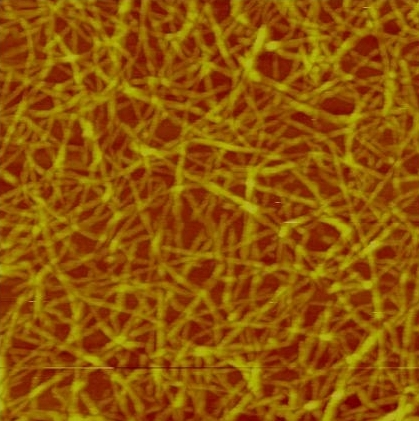
\includegraphics[width=0.5\linewidth]{img/AFM_Innventia_nanocellulose}
\caption{Fibrils of carboxymethylated nanocellulose adsorbed on a silica surface. \cite{xxx}}
\label{fig:cellulose}
\end{figure}




\subsection{Modeling the fibrils as a pinned line incidence system}



The cross-linking of microfibrils can be modeled using 2-dimensional pinned line incidence constraint system. 

%TODO system? problem?
\begin{definition} [2-Dimensional Pinned Line Incidence Graph] \label{prob:pinned_subspace}
A simple graph $G=(V,E)$ is a 2-dimensional pinned line incidence graph, 
if there is  a  set $X$ of $|E|$ pins with fixed positions in $\mathbb{R}^2$,
such that  every edge $e \in E$ corresponds to a pin $x \in X$ where $e$ is constrained to lie on a line passing through $x$.
%There exists a set $X$ of $|E|$ pins fixed in $\mathbb{R}^2$, such that each edge $e_i$

%Let $X$ be a  set of $m$ pins that are fixed in $\mathbb{R}^2$, and $V$ be the index set of a set of vertices. 
%For every pin $x \in X$, we are also given the indices of two vertices $v_1,v_2$ in $V$, 
%such that the line (edge) spanned by $v_1$ and $v_2$ must pass through $x$. 
% % % % % % % % % % % % % % % % % % %
%Find any such set of points $P$ satisfying the given incidences. 
%For every pin $x\in X$, we are also given a line $\supp{x}$, %of %a set of $s$-dimensional subspaces passing through 
%i.e, a size-two index subset of an unknown set of points $D = \{v_1,\ldots,v_n\}$ in $\mathbb{R}^2$, %$P = \{p_1,\ldots, p_n \}$, 
%such that  $x_i$ lies on the line spanned by $\supp{x}$. 
%%assume additionally that  
%%no $s$ pins lie on any single subspace defined by one of the above hyperedges.
%Find any such set D %$P[X]$ 
%that satisfies the given subspace incidences. % specified by $\supp[P]{x}$.%$\{S_i\}$. % on $P[X]$ and $X$.
\end{definition}



In the case of microfibril cross-linking, each fibril is 
attached to some fixed larger organelle/membrane at one spot, 
so it can be modeled as an edge/line segment incident at a pin in $X$. 
%For cross-linking density 2, 
%i.e.\ each fibril has two cross-linkings with other fibrils, 
The cross-linkings can be modeled as vertices in $V$.


\begin{figure}
\centering
\begin{subfigure}{.5\linewidth}
  \centering
  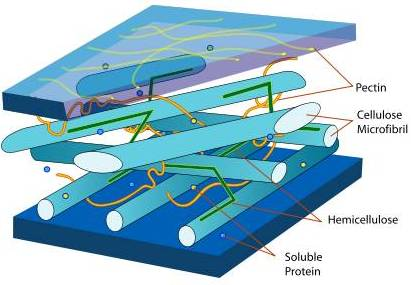
\includegraphics[width=\linewidth]{img/crosslink}
  \caption{}
  \label{fig:sub1}
\end{subfigure}%
\begin{subfigure}{.5\linewidth}
  \centering
  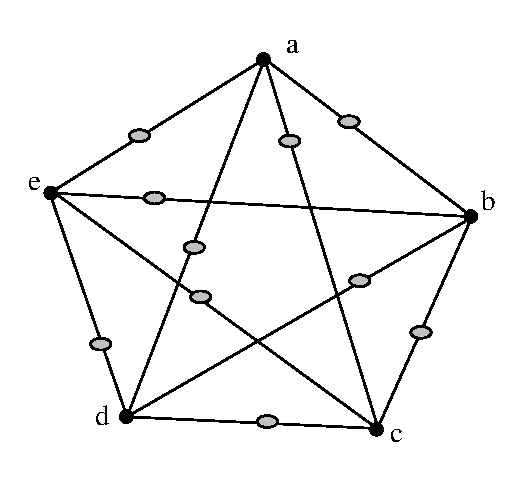
\includegraphics[width=.8\linewidth]{img/teq1}
  \caption{}
  \label{fig:sub2}
\end{subfigure}
\caption{(a) Cross-linking of microfibrils~\cite{xxx}. (b) A pinned line incidence graph.}
\label{fig:cross-linking}
\end{figure}


As an example, Figure~\ref{fig:cross-linking}, 
where the grey ovals stand for pins/attachments of fibrils and the black dots stand for vertices/cross-linkings.
There are 5 edges/fibrils,  and 10 vertices/cross-linkings in the graph.




\subsection{Optimal DR-plan for pinned line incidence systems}

%Recall the definitions in Section~\ref{priliminary}.

In this section, we will adapt the results in Section~\ref{xxx}
to give the Optimal DR-plan for 2-dimensional pinned line incidence graphs.
%The 2-dimensional pinned line incidence graphs and their DR-plans have 
Note the following differences from the bar-joint graphs: 

\begin{itemize}

\item For pinned line incidence graphs, all vertex weights are $2$, all edge weights are $1$, 
and the constant $k = 0$ \cite{xxxx}. 
%In other words, a pinned line incidence graph is well-constrained if $2|V| = |E|$ and $2|V'| \le |E'|$ for all induced non-trivial subgraphs $S=(V',E') \subseteq G$. 

\item 
\todo{Trivial graphs (must be overconstrained in the original definition) does not exist??? }\
\todo{Both a single vertex and a single edge are underconstrained}
\begin{itemize}

\item For  pinned line incidence graphs:
no trivial motion exists since the pins have fixed locations. 


\item 
\todo{We just define the %trivial graph/
DR-plan leaves for 2-dimensional pinned line incidence graphs to be single vertices...  }

\item \todo{A single edge can be a node of the DR-plan}

\end{itemize}


\item 
Notice that for pinned line incidence graphs, 
since the pins in $X$ have fixed positions on the plane, 
a well-constrained vertex-maximal proper subgraphs can be disconnected.\\
Without loss of generality, 
we slightly modify the requirement of DR-plan for pinned line incidence graphs
such that only connected subgraphs can be considered as a node of the DR-plan.

\end{itemize}


With the above modification, 
it is not hard to adapt Theorem~\ref{t1} %, the optimal DR-plan for 2-dimensional bar-joint graphs,
to show the structure of optimal DR-plan for 2-dimensional pinned line incidence graphs.


\begin{corollary}
Given a well-constrained 2-dimensional pinned line incidence graph, for node $C$ in $OptimalDRP(G)$ and the children of $C$ in $CompleteDRP(C)$ labeled as $C_1,\ldots,C_N$
\begin{enumerate}
    \item if $C_i \cap C_j$ is trivial then all $C_1,\ldots,C_N$ are children of $C$ in $OptimalDRP(G)$
    \item if $C_i \cap C_j$ is well-constrained then any two out of $C_1,\ldots,C_N$ will be the only children of $C$ in $OptimalDRP(G)$.
\end{enumerate}
\label{cor:pinned}
\end{corollary}

\todo{All Lemmas before Lemma 8 are proved with respect to general constraint systems,
and they go through for 2-dimensional pinned line incidence as well (without trivial graph??). }




Now we  show that Lemma 8 also holds for 2-dimensional pinned line incidence graphs. 

\begin{proof}[Proof of Lemma~\ref{wc-l3} for 2D pinned line incidence graphs]
We use the same notations as in the proof of Lemma~\ref{wc-c1} in Section~\ref{xxx}.
\begin{itemize}
    \item 4 cases: $C_k$ cannot be $Idc(C,R_i\cup R_j)$, $Idc(C,R'_i\cup R_j)$, $Idc(C,R_i\cup R'_j)$, or $Idc(C,R'_i\cup R'_j)$ because these are all disconnected (Corollary~\ref{wc-c1}) and by our modified requirement of DR-plan nodes.

%    \item 1 case: $C_k=Idc(C,R'_i\cup R'_j\cup D_{i,j})$ is not possible. Since $C_k\cup C_i = Idc(C,R'_i\cup R_j\cup D_{i,j})\neq C$ we have from Lemma \ref{wc-l2} that $C_k\cup C_i$ cannot be well-constrained. We also know it cannot be trivial because it contains well-constrained subgraphs. This means it must be under-constrained. From Lemma \ref{uc-l1}, we know that $C_k\cap C_i=Idc(C,R'_j\cup D_{i,j})$ must then be trivial. This is impossible because $D_{i,j}$ is well-constrained, thereby contradicting the assumption that $C_k$ is well-constrained.
%
%    \item 1 case: \todo{Uses 2D requirement:} $C_k=Idc(C,R'_i\cup R'_j\cup D'_{i,j})$ is not possible. The union with $C_i$ (or $C_j$) is not equal to $C$. Therefore, the union must be under-constrained which means the intersection must be trivial (a single node). However, $C_k\cap C_i=Idc(C,R'_j\cup D'_{i,j})$ and since $R'_j$ and $D'_{i,j}$ are not empty sets, it cannot be trivial making a contradiction.
%
%    \item 2 cases: \todo{Uses 2D requirement:} $C_k=Idc(C,R'_i\cup R_j\cup D'_{i,j})$ and $C_k=Idc(C,R_i\cup R'_j\cup D'_{i,j})$ are not possible. The proof mirrors the previous case, except you must choose $C_i$ and $C_j$, respectively, here.
\end{itemize}

\todo{All other cases are similar to the original proof.}

\end{proof}

%How theorems go through when only considering connected rigidity components

Given Lemma~\ref{wc-l3}, Lemma~\ref{uc-l2}, Theorem~\ref{uc-t1} and \ref{wc-t1} also apply to  2-dimensional pinned line incidence graphs,
proving Corollary~\ref{cor:pinned}. 

Therefore, we can analyze microfibril cross-linkings by finding the optimal DR-plan for  2-dimensional pinned line incidence graphs in the same way as for 2-dimensional bar-joint graphs.
 


